\documentclass{article}

\usepackage{arxiv}

\usepackage[utf8]{inputenc} % allow utf-8 input
\usepackage[T1]{fontenc}    % use 8-bit T1 fonts
\usepackage{hyperref}       % hyperlinks
\usepackage{url}            % simple URL typesetting
\usepackage{booktabs}       % professional-quality tables
\usepackage{amsfonts}       % blackboard math symbols
\usepackage{nicefrac}       % compact symbols for 1/2, etc.
\usepackage{microtype}      % microtypography
\usepackage{lipsum}		% Can be removed after putting your text content
\usepackage{graphicx}
\usepackage{doi}

\usepackage[backend=biber,sorting=none]{biblatex}
\addbibresource{references.bib}

\title{Reduce, Reuse, Reinterpret: an end-to-end pipeline workflow for particle physics}

%\date{September 9, 1985}	% Here you can change the date presented in the paper title
%\date{} 					% Or removing it

\author{ \href{https://orcid.org/0000-0001-6616-3433}{
\includegraphics[scale=0.06]{orcid.pdf}\hspace{1mm}Giordon~Stark}\thanks{More information...} \\
  University of California, Santa Cruz \\
  Santa Cruz Institute for Particle Physics, \\
  Interdisciplinary Sciences Building, Room \#337, 1156 High Street \\
  Santa Cruz, CA 95064 \\
	\texttt{gistark@ucsc.edu} \\
	%% examples of more authors
	\and
	\href{https://orcid.org/0000-0001-8392-0934}{
\includegraphics[scale=0.06]{orcid.pdf}\hspace{1mm}Mike~Hance} \\
  University of California, Santa Cruz \\
  Santa Cruz Institute for Particle Physics, \\
  Natural Sciences 2, Room \#317, 1156 High Street \\
  Santa Cruz, CA 95064 \\
	\texttt{mhance@ucsc.edu} \\
	%% \AND
	%% Coauthor \\
	%% Affiliation \\
	%% Address \\
	%% \texttt{email} \\
	%% \and
	%% Coauthor \\
	%% Affiliation \\
	%% Address \\
	%% \texttt{email} \\
	%% \and
	%% Coauthor \\
	%% Affiliation \\
	%% Address \\
	%% \texttt{email} \\
}

% Uncomment to remove the date
%\date{}

% Uncomment to override  the `A preprint' in the header
%\renewcommand{\headeright}{Technical Report}
%\renewcommand{\undertitle}{Technical Report}
\renewcommand{\shorttitle}{\textit{mapyde} - an end-to-end pipeline workflow for particle physics}

%%% TODO
%%% Add PDF metadata to help others organize their library
%%% Once the PDF is generated, you can check the metadata with
%%% $ pdfinfo template.pdf
\hypersetup{
  pdftitle={mapyde - an end-to-end pipeline workflow for particle physics},
  pdfsubject={q-bio.NC, q-bio.QM},
  pdfauthor={Giordon~Stark, Mike~Hance},
  pdfkeywords={First keyword, Second keyword, More},
}

\begin{document}
\maketitle

\begin{abstract}
Searches for new physics at the Large Hadron Collider have constrained many models of physics beyond the Standard Model.  Many searches also provide resources that allow them to be reinterpreted in the context of other models.  We demonstrate a pipeline that constrains previously untested models of new physics using supplementary information from ATLAS SUSY searches such as public analysis routines and serialized likelihoods.  These resources are combined with common event generation and simulation toolkits \textsc{MadGraph}, \textsc{Pythia}, and \textsc{Delphes} into workflows steered by \textsc{TOML} configuration files, and packaged as the \texttt{mapyde} python package.  The use of \texttt{mapyde} is demonstrated by constraining SUSY models with compressed sleptons and electroweakinos using ATLAS results.
\end{abstract}


%% %% keywords can be removed
%% \keywords{First keyword \and Second keyword \and More}


\section{Introduction}
\label{sec:introduction}

\begin{itemize}
\item Describe the reinterpretation problem.
\item Mention other toolkits:
  \begin{itemize}
  \item Full reinterpretation: RECAST
  \item Simplified likelihoods: GAMBIT? CHECKMATE?
  \item Others?
  \end{itemize}
\item Describe mapyde's approach
\item Paragraph describing this paper
\end{itemize}

\section{The \texttt{mapyde} toolkit}
\label{sec:mapyde}

\begin{itemize}
\item Tools:
  \begin{itemize}
  \item General tools: Madgraph, Pythia, Delphes
  \item ATLAS tools: SA
  \item Fits: pyhf
  \end{itemize}
\item Configuration: TOML files
\item Runtime:
  \begin{itemize}
  \item Docker containers
  \item Python steering
  \end{itemize}
\item Outputs
\end{itemize}

\section{Reinterpreting Compressed SUSY Searches from ATLAS}
\label{sec:reinterp}

\subsection{Implementation}
\label{sec:reinterp-imp}

\begin{itemize}
\item \texttt{mapyde} setup
\item MG+PY setup, versions, etc
\item ATLAS lepton efficiencies and the delphes card
\item Simpleanalysis routine, delphes2SA, sa2json
\item Public likelihoods
\end{itemize}

\subsection{Compressed Sleptons}
\label{reinterp-slep}

\begin{itemize}
\item Cross sections, k-factors
\item Acceptance checks
\item Reproducing ATLAS results
\item Describing the slepton-wino-bino model

\begin{figure}
	\centering
  \includegraphics[width=0.5\textwidth]{{./figures/feynman/output/slepton_wino_bino}}
	\caption{Feynman Diagram of Slepton-Wino-Bino.}
	\label{fig:feynman:slepton_wino_bino}
\end{figure}

\item Results
\end{itemize}

\begin{figure}
  \centering
  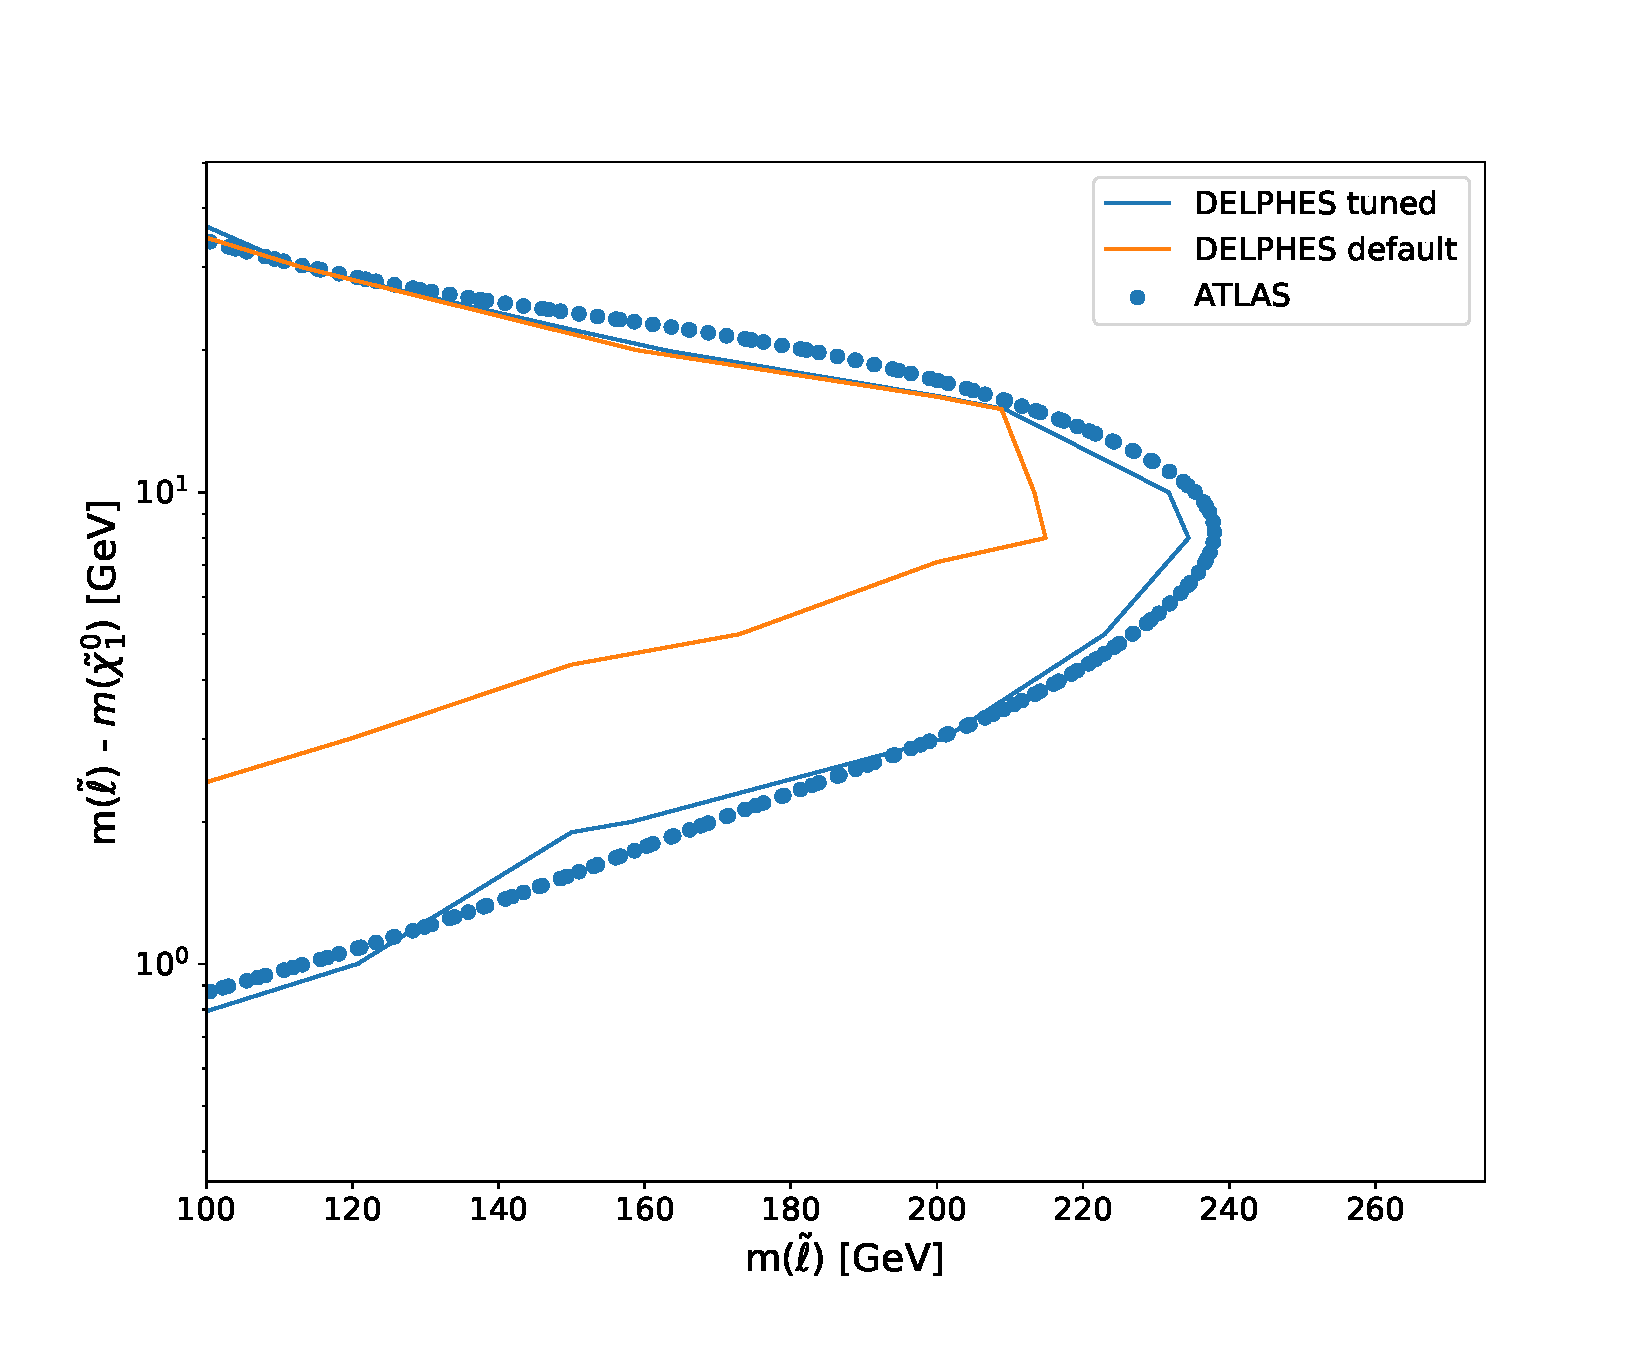
\includegraphics[width=0.48\textwidth]{{./figures/SleptonBino}}
  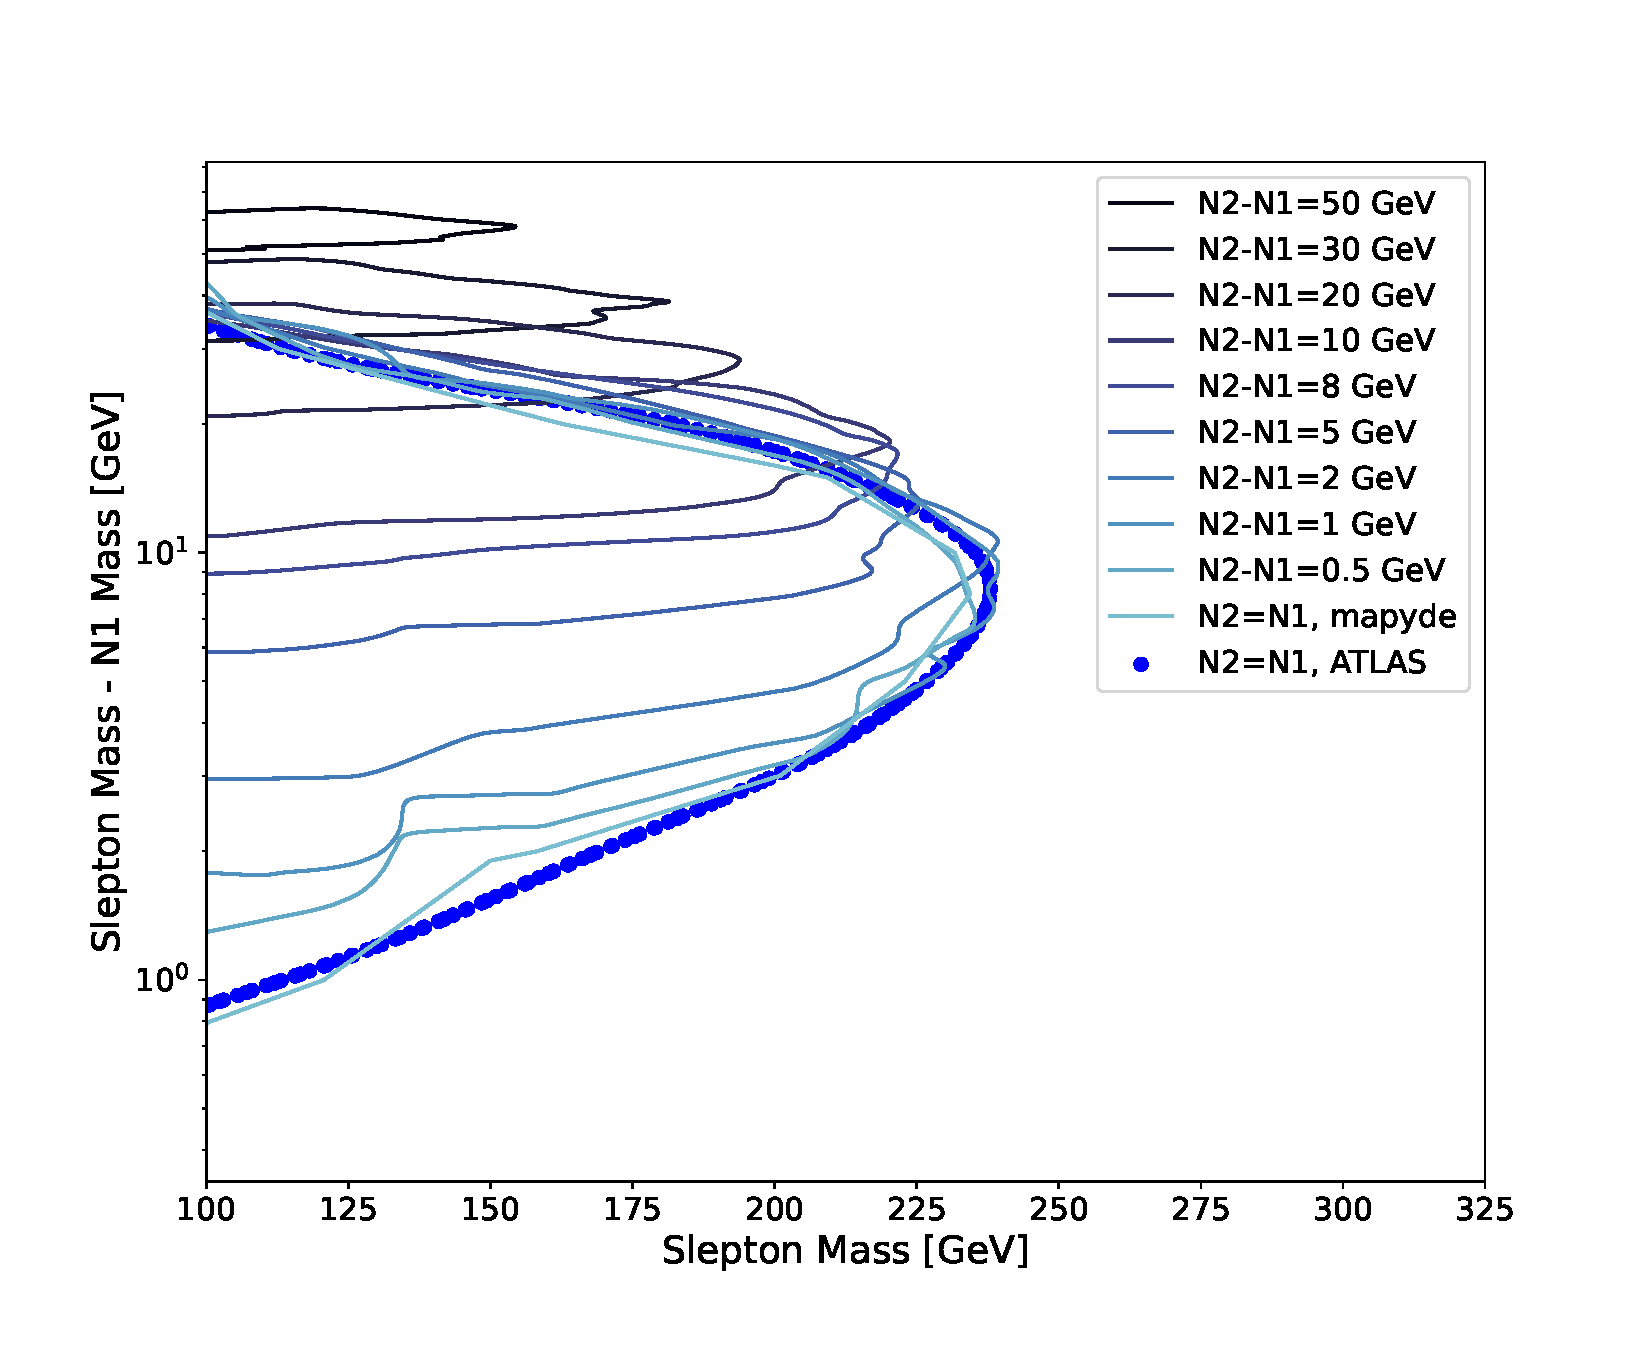
\includegraphics[width=0.48\textwidth]{{./figures/SleptonWinoBino}}
  \caption{Slepton limits}
  \label{fig:SleptonWinoBino}
\end{figure}


\subsection{Compressed Electroweakinos}
\label{reinterp-ewkino}

\begin{itemize}
\item Reproducing ATLAS results
\item Describing the higgsino-wino-bino model
\item Results
\end{itemize}

\begin{figure}
  \centering
  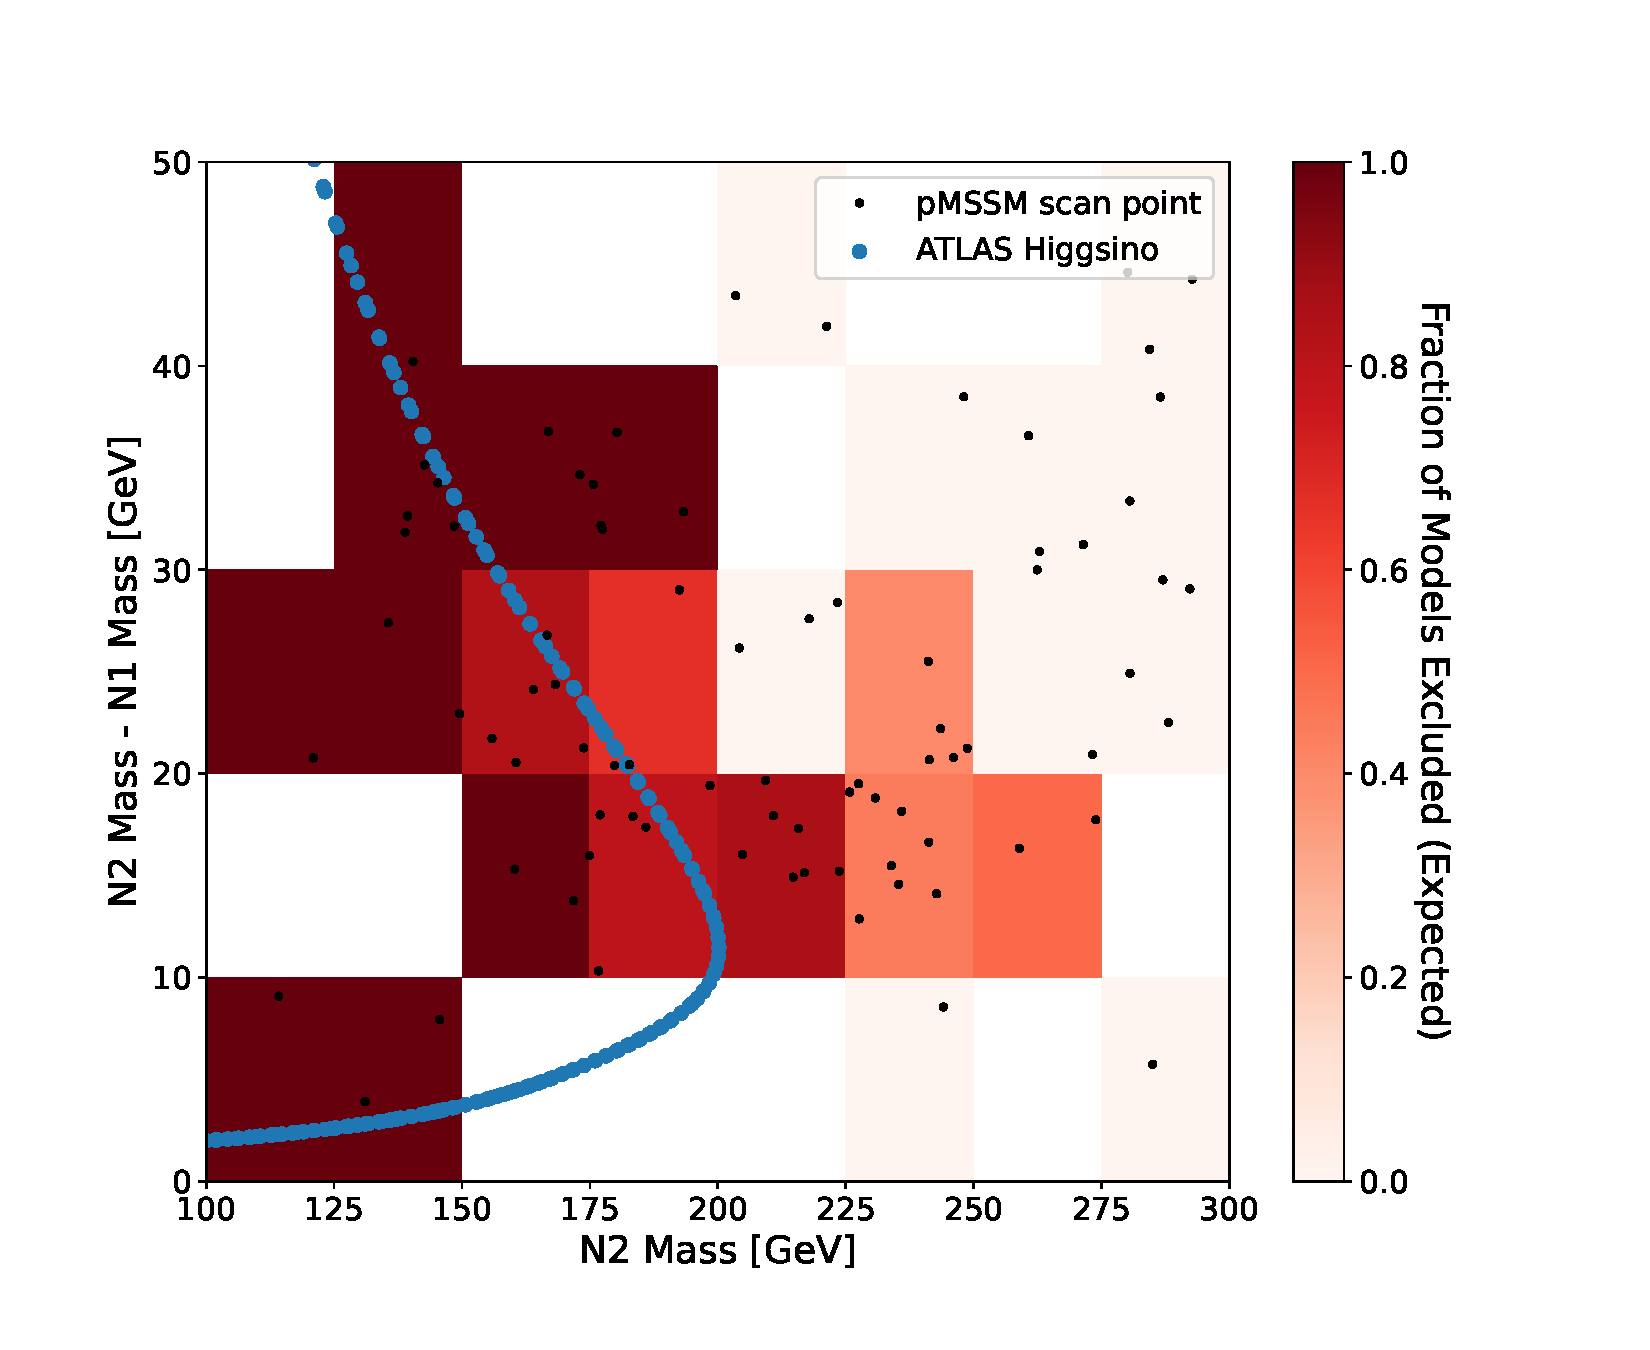
\includegraphics[width=0.8\textwidth]{{./figures/EWKino_pmssm}}
  \caption{Electroweakino limits}
  \label{fig:EWKino_pmssm}
\end{figure}

\section{Conclusion}

We have presented \texttt{mapyde}, shown some reinterpretations, and we're done.

\printbibliography

\end{document}
